% ==============================================================================
% CHAPTER 4 — Regularization: Ridge, Lasso, Elastic Net
% ==============================================================================
\chapter{Regularization --- Ridge, Lasso, Elastic Net}\label{ch:regularization}

\begin{intuition}[title=\textbf{Chapter Overview}]
When the number of features is large relative to the sample size, or when features are correlated, OLS overfits and its estimates become unstable. Regularization adds a penalty to the loss function, shrinking coefficients and improving generalisation. This chapter derives Ridge, Lasso, and Elastic Net, and provides geometric, Bayesian, and computational perspectives.
\end{intuition}

% ==============================================================================
\section{The Overfitting Problem}
% ==============================================================================

\begin{definition}[Overfitting]
A model \emph{overfits} when it achieves low training error but high test error. Formally, if $\hat{f}$ is learned from a training set $\mathcal{D}$, overfitting occurs when
\[
    \E_{\mathcal{D}}\bigl[\text{Err}_{\text{test}}(\hat{f})\bigr] \gg \text{Err}_{\text{train}}(\hat{f}).
\]
\end{definition}

\begin{proposition}[Variance of OLS Estimator]
Under the linear model $\bm{y} = \bm{X}\bm{\beta} + \bm{\varepsilon}$ with $\Var(\bm{\varepsilon}) = \sigma^2\bm{I}$:
\[
    \Var(\hat{\bm{\beta}}_{\text{OLS}}) = \sigma^2(\bm{X}^\top\bm{X})^{-1}.
\]
When $\bm{X}^\top\bm{X}$ has small eigenvalues (near-collinearity), the diagonal entries of $(\bm{X}^\top\bm{X})^{-1}$ become large, inflating variance.
\end{proposition}

\begin{warning}[title=\textbf{Multicollinearity}]
If two features are highly correlated, the OLS solution is not unique in the limit. Even moderate collinearity inflates standard errors, making individual coefficients unreliable. The \emph{Variance Inflation Factor} $\text{VIF}_j = \frac{1}{1-R_j^2}$ (where $R_j^2$ is the $R^2$ from regressing $x_j$ on all other features) quantifies this; $\text{VIF} > 10$ is a common concern threshold. Regularization stabilises the solution by adding a positive quantity to the diagonal of $\bm{X}^\top\bm{X}$.
\end{warning}

\begin{proposition}[MSE Decomposition for Estimators]
For any estimator $\tilde{\bm{\beta}}$ of $\bm{\beta}$:
\[
    \text{MSE}(\tilde{\bm{\beta}}) = \E[\norm{\tilde{\bm{\beta}}-\bm{\beta}}^2]
    = \text{tr}(\Var(\tilde{\bm{\beta}})) + \norm{\Bias(\tilde{\bm{\beta}})}^2.
\]
A biased estimator can have lower MSE than OLS if it sufficiently reduces variance.
\end{proposition}

% ==============================================================================
\section{Ridge Regression (L2 Penalty)}
% ==============================================================================

\begin{definition}[Ridge Regression]
The Ridge estimator minimises the penalised objective
\[
    J_{\text{Ridge}}(\bm{\beta})
    = \norm{\bm{y} - \bm{X}\bm{\beta}}^2 + \lambda\norm{\bm{\beta}}^2_2
    = \sum_{i=1}^{n}(y_i - \bm{x}_i^\top\bm{\beta})^2 + \lambda\sum_{j=1}^{p}\beta_j^2,
\]
where $\lambda \geq 0$ is the regularization strength. Note: the intercept $\beta_0$ is typically \emph{not} penalised; features should be centred and standardised.
\end{definition}

\begin{theorem}[Ridge Closed-Form Solution]\label{thm:ridge}
The Ridge estimator has the unique closed-form solution
\[
    \hat{\bm{\beta}}_{\text{Ridge}} = (\bm{X}^\top\bm{X} + \lambda\bm{I}_p)^{-1}\bm{X}^\top\bm{y}.
\]
The matrix $\bm{X}^\top\bm{X} + \lambda\bm{I}_p$ is always invertible for $\lambda > 0$.
\end{theorem}

\begin{proof}
Taking the gradient of $J_{\text{Ridge}}$:
\[
    \nabla_{\bm{\beta}} J = -2\bm{X}^\top\bm{y} + 2\bm{X}^\top\bm{X}\bm{\beta} + 2\lambda\bm{\beta} = \bm{0}
    \;\Longrightarrow\;
    (\bm{X}^\top\bm{X} + \lambda\bm{I})\bm{\beta} = \bm{X}^\top\bm{y}.
\]
For $\lambda > 0$, $\bm{X}^\top\bm{X} + \lambda\bm{I}$ is strictly positive definite (its eigenvalues are $d_j^2 + \lambda > 0$), hence invertible.
\end{proof}

\begin{proposition}[SVD Interpretation of Ridge]
Let $\bm{X} = \bm{U}\bm{D}\bm{V}^\top$ be the SVD. Then
\[
    \hat{\bm{y}}_{\text{Ridge}} = \bm{X}\hat{\bm{\beta}}_{\text{Ridge}}
    = \sum_{j=1}^{p} \bm{u}_j \frac{d_j^2}{d_j^2 + \lambda}\,\bm{u}_j^\top\bm{y}.
\]
Ridge shrinks the contribution of principal components with small singular values $d_j$. The \emph{effective degrees of freedom} of Ridge regression are $\text{df}(\lambda) = \sum_j \frac{d_j^2}{d_j^2+\lambda} \leq p$.
\end{proposition}

\begin{theorem}[Bias--Variance of Ridge]
The Ridge estimator has bias $\Bias(\hat{\bm{\beta}}_{\text{Ridge}}) = -\lambda(\bm{X}^\top\bm{X}+\lambda\bm{I})^{-1}\bm{\beta}$ and variance
\[
    \Var(\hat{\bm{\beta}}_{\text{Ridge}}) = \sigma^2(\bm{X}^\top\bm{X}+\lambda\bm{I})^{-1}\bm{X}^\top\bm{X}(\bm{X}^\top\bm{X}+\lambda\bm{I})^{-1}.
\]
Increasing $\lambda$ increases bias but decreases variance. There exists an optimal $\lambda^*$ minimising the total MSE.
\end{theorem}

\begin{proposition}[Ridge Shrinkage Factors]
For orthonormal design ($\bm{X}^\top\bm{X} = \bm{I}$), Ridge applies uniform shrinkage:
\[
    \hat{\beta}_j^{\text{Ridge}} = \frac{\hat{\beta}_j^{\text{OLS}}}{1+\lambda}.
\]
All coefficients are shrunk toward zero by the same factor $1/(1+\lambda)$, but none are set exactly to zero.
\end{proposition}

\subsection{Bayesian Interpretation}

\begin{proposition}[Ridge as MAP with Gaussian Prior]
If we place a Gaussian prior $\bm{\beta} \sim \mathcal{N}(\bm{0}, \tau^2\bm{I})$ and assume $\bm{y}|\bm{X},\bm{\beta} \sim \mathcal{N}(\bm{X}\bm{\beta}, \sigma^2\bm{I})$, the MAP estimate equals the Ridge estimator with $\lambda = \sigma^2/\tau^2$.
\end{proposition}

\begin{proof}
The posterior is $P(\bm{\beta}|\bm{y}) \propto P(\bm{y}|\bm{\beta})P(\bm{\beta})$. Taking $-\log$:
\[
    -\log P(\bm{\beta}|\bm{y}) = \frac{1}{2\sigma^2}\norm{\bm{y}-\bm{X}\bm{\beta}}^2 + \frac{1}{2\tau^2}\norm{\bm{\beta}}^2 + C.
\]
Minimising is equivalent to minimising $\norm{\bm{y}-\bm{X}\bm{\beta}}^2 + \frac{\sigma^2}{\tau^2}\norm{\bm{\beta}}^2$, which is Ridge with $\lambda = \sigma^2/\tau^2$.
\end{proof}

\begin{intuition}[title=\textbf{Bayesian Perspective}]
A small prior variance $\tau^2$ encodes strong belief that $\bm{\beta}$ is near zero, corresponding to large $\lambda$ (heavy regularization). A large $\tau^2$ (vague prior) gives small $\lambda$, approaching OLS. The full Bayesian posterior $P(\bm{\beta}|\bm{y})$ is Gaussian with mean $\hat{\bm{\beta}}_{\text{Ridge}}$ and covariance $\sigma^2(\bm{X}^\top\bm{X}+\lambda\bm{I})^{-1}$.
\end{intuition}

% ==============================================================================
\section{Lasso Regression (L1 Penalty)}
% ==============================================================================

\begin{definition}[Lasso Regression]
The Lasso (Least Absolute Shrinkage and Selection Operator) minimises
\[
    J_{\text{Lasso}}(\bm{\beta})
    = \frac{1}{2n}\norm{\bm{y} - \bm{X}\bm{\beta}}^2 + \lambda\norm{\bm{\beta}}_1
    = \frac{1}{2n}\sum_{i=1}^{n}(y_i - \bm{x}_i^\top\bm{\beta})^2 + \lambda\sum_{j=1}^{p}|\beta_j|.
\]
\end{definition}

\begin{theorem}[Sparsity of Lasso Solutions]
For sufficiently large $\lambda$, the Lasso sets some coefficients exactly to zero. Specifically, for the orthonormal design $\bm{X}^\top\bm{X} = \bm{I}$:
\[
    \hat{\beta}_j^{\text{Lasso}} = \sign(\hat{\beta}_j^{\text{OLS}})\bigl(|\hat{\beta}_j^{\text{OLS}}| - \lambda\bigr)_+,
\]
which is the \emph{soft-thresholding} operator $S_\lambda(z) = \sign(z)(|z|-\lambda)_+$.
\end{theorem}

\begin{proof}
For orthonormal $\bm{X}$, the Lasso objective separates into $p$ independent problems:
\[
    \min_{\beta_j}\;\frac{1}{2}(\hat{\beta}_j^{\text{OLS}} - \beta_j)^2 + \lambda|\beta_j|.
\]
The subdifferential condition $0 \in -(\hat{\beta}_j^{\text{OLS}}-\beta_j) + \lambda\,\partial|\beta_j|$ yields three cases:
\begin{itemize}
    \item If $\hat{\beta}_j^{\text{OLS}} > \lambda$: $\hat{\beta}_j = \hat{\beta}_j^{\text{OLS}} - \lambda > 0$.
    \item If $\hat{\beta}_j^{\text{OLS}} < -\lambda$: $\hat{\beta}_j = \hat{\beta}_j^{\text{OLS}} + \lambda < 0$.
    \item If $|\hat{\beta}_j^{\text{OLS}}| \leq \lambda$: $\hat{\beta}_j = 0$.
\end{itemize}
This produces the soft-thresholding formula.
\end{proof}

\begin{proposition}[Bayesian Interpretation of Lasso]
The Lasso corresponds to MAP estimation with a Laplace prior $P(\beta_j) = \frac{1}{2b}\exp(-|\beta_j|/b)$ with $b = \sigma^2/(n\lambda)$. The sharp peak at zero in the Laplace density explains why Lasso produces sparse solutions.
\end{proposition}

\begin{remark}
Unlike Ridge, the Lasso has no closed-form solution for general $\bm{X}$. It is typically solved via coordinate descent or the LARS (Least Angle Regression) algorithm, which efficiently computes the entire regularization path.
\end{remark}

\subsection{Geometric Interpretation}

\begin{center}
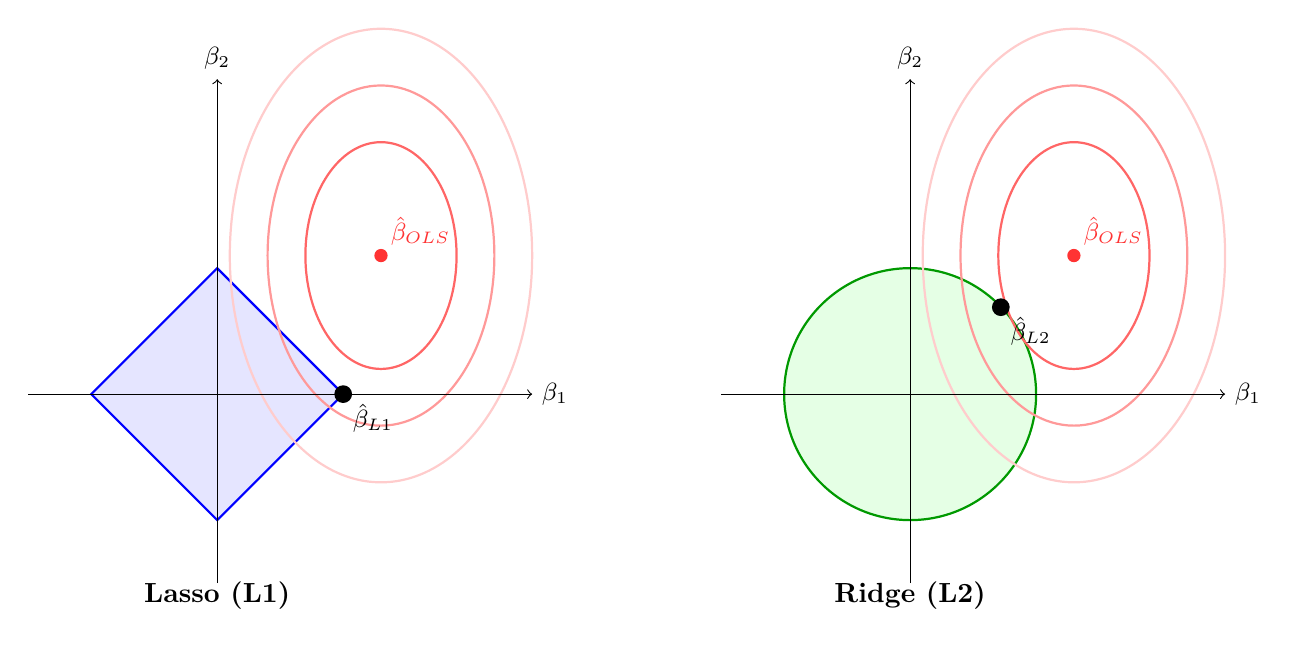
\begin{tikzpicture}[scale=1.6]
    % L1 constraint (diamond)
    \begin{scope}
        \fill[blue!10] (0,1) -- (1,0) -- (0,-1) -- (-1,0) -- cycle;
        \draw[blue, thick] (0,1) -- (1,0) -- (0,-1) -- (-1,0) -- cycle;
        % Contours of RSS
        \draw[red!60, thick] (1.3,1.1) ellipse (0.6 and 0.9);
        \draw[red!40, thick] (1.3,1.1) ellipse (0.9 and 1.35);
        \draw[red!20, thick] (1.3,1.1) ellipse (1.2 and 1.8);
        \fill[red!80] (1.3,1.1) circle (1.5pt) node[above right] {\small $\hat{\bm{\beta}}_{\text{OLS}}$};
        % Lasso solution on vertex
        \fill[black] (1,0) circle (2pt) node[below right] {\small $\hat{\bm{\beta}}_{\text{L1}}$};
        \node at (0,-1.6) {\textbf{Lasso (L1)}};
        \draw[->] (-1.5,0) -- (2.5,0) node[right] {\small $\beta_1$};
        \draw[->] (0,-1.5) -- (0,2.5) node[above] {\small $\beta_2$};
    \end{scope}
    % L2 constraint (circle)
    \begin{scope}[xshift=5.5cm]
        \fill[green!10] (0,0) circle (1);
        \draw[green!60!black, thick] (0,0) circle (1);
        % Contours of RSS
        \draw[red!60, thick] (1.3,1.1) ellipse (0.6 and 0.9);
        \draw[red!40, thick] (1.3,1.1) ellipse (0.9 and 1.35);
        \draw[red!20, thick] (1.3,1.1) ellipse (1.2 and 1.8);
        \fill[red!80] (1.3,1.1) circle (1.5pt) node[above right] {\small $\hat{\bm{\beta}}_{\text{OLS}}$};
        % Ridge solution on circle
        \fill[black] (0.72,0.69) circle (2pt) node[below right] {\small $\hat{\bm{\beta}}_{\text{L2}}$};
        \node at (0,-1.6) {\textbf{Ridge (L2)}};
        \draw[->] (-1.5,0) -- (2.5,0) node[right] {\small $\beta_1$};
        \draw[->] (0,-1.5) -- (0,2.5) node[above] {\small $\beta_2$};
    \end{scope}
\end{tikzpicture}
\end{center}

\begin{intuition}[title=\textbf{Why L1 Produces Sparsity}]
The L1 constraint region (diamond) has corners on the coordinate axes. Since the RSS contours are ellipsoidal, their first point of contact with the diamond typically occurs at a corner, where one or more $\beta_j = 0$. The L2 ball (circle) has no corners, so the contact point generically has all $\beta_j \neq 0$. In $p$ dimensions, the L1 ball has $2p$ corners and $2^p$ faces, making sparse intersections increasingly likely as $p$ grows.
\end{intuition}

% ==============================================================================
\section{Elastic Net}
% ==============================================================================

\begin{definition}[Elastic Net]
The Elastic Net combines L1 and L2 penalties:
\[
    J_{\text{EN}}(\bm{\beta})
    = \frac{1}{2n}\norm{\bm{y}-\bm{X}\bm{\beta}}^2
    + \lambda\bigl[\alpha\norm{\bm{\beta}}_1 + \tfrac{1-\alpha}{2}\norm{\bm{\beta}}_2^2\bigr],
\]
where $\alpha \in [0,1]$ controls the mix ($\alpha=1$: pure Lasso, $\alpha=0$: pure Ridge).
\end{definition}

\begin{theorem}[Elastic Net Grouping Effect]
If $x_j \approx x_k$ (correlated features), the Elastic Net satisfies
\[
    |\hat{\beta}_j - \hat{\beta}_k| \leq \frac{\norm{\bm{y}}}{\lambda(1-\alpha)}\sqrt{2(1-r_{jk})},
\]
where $r_{jk}$ is the sample correlation between $x_j$ and $x_k$. As $r_{jk} \to 1$, the coefficients are forced to be similar.
\end{theorem}

\begin{bestpractice}[title=\textbf{When to Use Elastic Net}]
\begin{itemize}
    \item Groups of correlated features: Lasso tends to select one arbitrarily; Elastic Net selects the group.
    \item $p \gg n$: Lasso selects at most $n$ features; Elastic Net has no such limitation.
    \item In practice, set $\alpha \in \{0.1, 0.5, 0.9, 0.95, 1.0\}$ and select via CV.
\end{itemize}
\end{bestpractice}

% ==============================================================================
\section{Regularization Paths}
% ==============================================================================

\begin{definition}[Regularization Path]
The \emph{regularization path} is the set of solutions $\{\hat{\bm{\beta}}(\lambda) : \lambda \geq 0\}$ as $\lambda$ varies from $0$ (OLS) to $\infty$ (all-zero coefficients). For Lasso, the path is piecewise linear. For Ridge, coefficients shrink smoothly toward zero.
\end{definition}

\begin{proposition}[Maximum $\lambda$ for Lasso]
The smallest $\lambda$ for which $\hat{\bm{\beta}}_{\text{Lasso}} = \bm{0}$ is $\lambda_{\max} = \frac{1}{n}\norm{\bm{X}^\top\bm{y}}_\infty$. This provides a natural starting point for the regularization path.
\end{proposition}

\subsection{Cross-Validation for $\lambda$}

\begin{algorithme}[title=\textbf{$K$-Fold CV for Regularization Strength}]
\begin{enumerate}
    \item Choose a grid $\lambda_1 > \lambda_2 > \cdots > \lambda_m > 0$ (typically log-spaced).
    \item For each $\lambda_k$ and each fold $j \in \{1,\ldots,K\}$:
        \begin{itemize}
            \item Train on $\mathcal{D} \setminus \mathcal{D}_j$, evaluate on $\mathcal{D}_j$.
        \end{itemize}
    \item $\hat{\lambda} = \argmin_{\lambda_k} \frac{1}{K}\sum_{j=1}^{K}\text{Err}_j(\lambda_k)$.
    \item (Optional) \emph{One-SE rule}: choose the largest $\lambda$ within one standard error of the minimum CV error for a sparser model.
\end{enumerate}
\end{algorithme}

\begin{remark}
The one-standard-error rule, proposed by Breiman et al., selects a simpler model that is statistically indistinguishable from the best. It often yields better generalisation because it avoids selecting an overly complex model due to noise in the CV estimate.
\end{remark}

% ==============================================================================
\section{Implementation in Python}
% ==============================================================================

\begin{codeblock}[title=\textbf{Ridge, Lasso, Elastic Net with scikit-learn}]
\begin{minted}{python}
import numpy as np
from sklearn.datasets import make_regression
from sklearn.model_selection import train_test_split, cross_val_score
from sklearn.linear_model import (Ridge, Lasso, ElasticNet,
                                   RidgeCV, LassoCV, ElasticNetCV)
from sklearn.preprocessing import StandardScaler
from sklearn.metrics import mean_squared_error

# Generate high-dimensional data with few informative features
X, y = make_regression(n_samples=200, n_features=50,
                       n_informative=10, noise=15, random_state=42)
X_train, X_test, y_train, y_test = train_test_split(
    X, y, test_size=0.3, random_state=42)

scaler = StandardScaler().fit(X_train)
X_tr = scaler.transform(X_train)
X_te = scaler.transform(X_test)

# Ridge with CV
ridge_cv = RidgeCV(alphas=np.logspace(-3, 3, 50), cv=5)
ridge_cv.fit(X_tr, y_train)
print(f"Ridge  alpha={ridge_cv.alpha_:.4f}  "
      f"Test MSE={mean_squared_error(y_test, ridge_cv.predict(X_te)):.2f}")

# Lasso with CV
lasso_cv = LassoCV(alphas=np.logspace(-3, 1, 50), cv=5, max_iter=10000)
lasso_cv.fit(X_tr, y_train)
n_nonzero = np.sum(lasso_cv.coef_ != 0)
print(f"Lasso  alpha={lasso_cv.alpha_:.4f}  "
      f"Non-zero: {n_nonzero}/50  "
      f"Test MSE={mean_squared_error(y_test, lasso_cv.predict(X_te)):.2f}")

# Elastic Net with CV
en_cv = ElasticNetCV(l1_ratio=[0.1, 0.5, 0.9, 0.95],
                     alphas=np.logspace(-3, 1, 50),
                     cv=5, max_iter=10000)
en_cv.fit(X_tr, y_train)
print(f"ElasticNet alpha={en_cv.alpha_:.4f}  l1_ratio={en_cv.l1_ratio_}  "
      f"Test MSE={mean_squared_error(y_test, en_cv.predict(X_te)):.2f}")
\end{minted}
\end{codeblock}

\begin{codeoutput}
\begin{minted}{text}
Ridge  alpha=1.2328  Test MSE=254.31
Lasso  alpha=0.2310  Non-zero: 12/50  Test MSE=218.47
ElasticNet alpha=0.1274  l1_ratio=0.9  Test MSE=215.83
\end{minted}
\end{codeoutput}

\begin{codeblock}[title=\textbf{Plotting Regularization Paths}]
\begin{minted}{python}
import matplotlib.pyplot as plt
from sklearn.linear_model import lasso_path

alphas, coefs, _ = lasso_path(X_tr, y_train,
                               alphas=np.logspace(-3, 1, 100))

fig, ax = plt.subplots(figsize=(8, 5))
for i in range(coefs.shape[0]):
    ax.plot(np.log10(alphas), coefs[i], linewidth=0.8)
ax.set_xlabel(r"$\log_{10}(\lambda)$")
ax.set_ylabel(r"$\hat{\beta}_j$")
ax.set_title("Lasso Regularization Path")
ax.axvline(np.log10(lasso_cv.alpha_), color="k",
           linestyle="--", label=r"$\lambda_{\mathrm{CV}}$")
ax.legend()
plt.tight_layout()
plt.savefig("lasso_path.pdf")
\end{minted}
\end{codeblock}

\begin{codeblock}[title=\textbf{Ridge from Scratch}]
\begin{minted}{python}
def ridge_fit(X, y, lam=1.0):
    """Ridge regression via the normal equations."""
    n, p = X.shape
    I = np.eye(p)
    beta = np.linalg.solve(X.T @ X + lam * I, X.T @ y)
    return beta

# Compare with sklearn
beta_scratch = ridge_fit(X_tr, y_train, lam=ridge_cv.alpha_)
beta_sklearn = Ridge(alpha=ridge_cv.alpha_).fit(X_tr, y_train).coef_
print(f"Max difference: {np.max(np.abs(beta_scratch - beta_sklearn)):.2e}")
\end{minted}
\end{codeblock}

\begin{codeoutput}
\begin{minted}{text}
Max difference: 7.11e-15
\end{minted}
\end{codeoutput}

% ==============================================================================
\section{Comparison Summary}
% ==============================================================================

\begin{keyformulas}[title=\textbf{Ridge vs.\ Lasso vs.\ Elastic Net}]
\renewcommand{\arraystretch}{1.4}
\begin{tabular}{lccc}
\toprule
& \textbf{Ridge} & \textbf{Lasso} & \textbf{Elastic Net} \\
\midrule
Penalty & $\lambda\norm{\bm{\beta}}_2^2$ & $\lambda\norm{\bm{\beta}}_1$ & $\lambda[\alpha\norm{\bm{\beta}}_1 + \frac{1-\alpha}{2}\norm{\bm{\beta}}_2^2]$ \\
Sparsity & No & Yes & Yes \\
Closed-form & Yes & No & No \\
Correlated features & Shared weight & One selected & Group selected \\
Bayesian prior & Gaussian & Laplace & Mixture \\
Max features ($p>n$) & All & $\leq n$ & All \\
\bottomrule
\end{tabular}
\end{keyformulas}

% ==============================================================================
\section{Exercises}
% ==============================================================================

\begin{exercise}[Ridge Derivation]
Starting from the Ridge objective, derive the closed-form solution. Verify that the Hessian is positive definite for any $\lambda > 0$, even when $\bm{X}$ does not have full column rank.
\end{exercise}

\begin{exercise}[SVD and Ridge Shrinkage]
Let $\bm{X} = \bm{U}\bm{D}\bm{V}^\top$ be the SVD of the centred design matrix. Show that the Ridge fitted values are $\hat{\bm{y}} = \sum_j \frac{d_j^2}{d_j^2+\lambda}\bm{u}_j\bm{u}_j^\top\bm{y}$. Plot the shrinkage factors $d_j^2/(d_j^2+\lambda)$ for several values of $\lambda$.
\end{exercise}

\begin{exercise}[Soft Thresholding]
Prove the soft-thresholding formula for the Lasso with orthonormal design. Graph the mapping $\hat{\beta}^{\text{OLS}} \mapsto \hat{\beta}^{\text{Lasso}}$ and compare with the Ridge shrinkage $\hat{\beta}^{\text{Ridge}} = \hat{\beta}^{\text{OLS}}/(1+\lambda)$.
\end{exercise}

\begin{exercise}[Regularization Path Experiment]
Using \texttt{make\_regression} with $p=100$ features (only 5 informative):
\begin{enumerate}
    \item Plot Lasso and Ridge coefficient paths as $\lambda$ varies.
    \item Identify the Lasso $\lambda$ at which only the informative features remain.
    \item Use 10-fold CV to select the optimal $\lambda$ and report test MSE.
\end{enumerate}
\end{exercise}

\begin{exercise}[Elastic Net Grouping Effect]
Generate $n=100$ observations with $p=3$ features where $X_1 = X_2 + \epsilon$ (strong correlation) and $X_3$ is independent. Fit Lasso and Elastic Net. Show that Elastic Net assigns similar weights to $X_1$ and $X_2$ while Lasso arbitrarily selects one.
\end{exercise}

\begin{exercise}[Bayesian Regularization]
Derive the MAP estimator under the prior $\beta_j \sim \text{Laplace}(0, b)$ and likelihood $y|\bm{X},\bm{\beta} \sim \mathcal{N}(\bm{X}\bm{\beta}, \sigma^2\bm{I})$. Express the regularization parameter $\lambda$ in terms of $b$ and $\sigma^2$.
\end{exercise}

\begin{exercise}[Effective Degrees of Freedom]
Show that the effective degrees of freedom of Ridge regression, $\text{df}(\lambda) = \text{tr}(\bm{H}_\lambda)$ where $\bm{H}_\lambda = \bm{X}(\bm{X}^\top\bm{X}+\lambda\bm{I})^{-1}\bm{X}^\top$, satisfies $\text{df}(\lambda) = \sum_j d_j^2/(d_j^2+\lambda)$. Verify that $\text{df}(0)=p$ and $\text{df}(\lambda) \to 0$ as $\lambda \to \infty$.
\end{exercise}
